\documentclass[a4paper, titlepage, oneside]{article}
\usepackage[australian]{babel}
\usepackage{csquotes}
\usepackage[vmargin = 2cm, hmargin = 2cm]{geometry}
\usepackage{amsmath,amssymb}
\usepackage{graphicx, epstopdf, listings, csvsimple, float, xcolor}
\usepackage[allcolors = blue, colorlinks = true, pdfpagemode = UseNone, pdfstartview = FitH]{hyperref}
\usepackage{multicol}
\usepackage{wasysym}
\usepackage[backend = biber, style = authoryear, alldates = iso8601]{biblatex}
\usepackage[cdot, amssymb]{SIunits}

% listings, xcolor
\lstset{language=Matlab,
    commentstyle=\color{gray}\textit,
    stringstyle=\color{purple},
    showstringspaces=false,
    numbers=left,
    breaklines=true,
    breakatwhitespace=true,
    aboveskip=0pt,
    belowskip=20pt}

% Bibliography setup
\renewcommand{\nameyeardelim}{\addcomma\addspace} % Change delimiter for in-line citations to include a comma
\addbibresource{group-report.bib}

% babel   : set language, for packages that need it
% csquotes  : context-sensitive quotes
% geometry  : page margins
% amsmath : maths
% amssymb : maths (\square redefined by siunits)
% graphicx  : \includegraphic
% epstopdf  : use of eps files in document
% hyperref  : in-document links
% listings  : import external code
% csvsimple : import csv tables
% float   : float graphics
% xcolor  : use colour formatting
% wasysym : \astrosun (conflict with amssymb)
% biblatex : bibliography
% siunits : management of SI units; encourage using \unit{value}{units} command whenever possible

% Custom commands
\newcommand{\elem}[2]{\textsuperscript{#1}{#2}}
\newcommand{\molec}[2]{\ensuremath{\text{#1}_{#2}}}
\newcommand{\e}[1]{\ensuremath{\times 10^{#1}}}
\newcommand{\smass}{\ensuremath{\mega_\odot}} % This hack relies on the SIunits package

% Document proper
\begin{document}
\title{\textbf{Searching for molecular gas towards TeV gamma-ray sources: Analysing 3D data cubes of the molecular gas tracer carbon monoxide with images from the HESS gamma-ray telescopes.}}
\author{A.~K. Child \and C.~M. Roe-Simons \and K.~T. Leaver \and H.~D. Poulter \and R.~M. Harvey}
\date{} %Leave blank to print no date, or you can type in the desired date
\maketitle

\setcounter{page}{1}
\pagenumbering{roman}
\numberwithin{equation}{section}

\tableofcontents

\clearpage
\setcounter{page}{1}
\pagenumbering{arabic}

\begin{center}
{\LARGE \textbf{Searching for molecular gas towards TeV gamma-ray sources: Analysing 3D data cubes of the molecular gas tracer carbon monoxide with images from the HESS gamma-ray telescopes.}}

\vspace{1.5em}

\textsc{A.~K. Child\footnote{Featured telescopes} \quad C.~M. Roe-Simons\footnote{Cosmic ray sources} \quad K.~T. Leaver\footnote{\elem{12}{CO} and \elem{13}{CO} as tracers} \quad H.~D. Poulter\footnote{Galactic rotation} \quad R.~M. Harvey\footnote{Molecular clouds and cosmic ray interactions}}
\end{center}

\vspace{2em}

\begin{minipage}{0.93\textwidth}
\begin{abstract}
This report is about finding the TeV sources and molecular clouds associated with such sources. It beings with a brief overview of the types of physical and astronomical concepts behind the science that has been used in writing up the report and making the conclusions. Bro!!
\end{abstract}
\end{minipage}

% \vspace{2.5em} % What the heck man this looks trash

\begin{multicols}{2}
\section{Introduction}
\paragraph{}
Words words words, quick run-down of gamma rays and really high ones, just pretty much do a Gavin and copy stuff from Gavin's slides and so on and so forth.

\section{Theory}
\paragraph{}
Theory stuff goes in here, including but not limited to:
\begin{itemize}
\item Cosmic ray sources
\item Large molecular clouds, and their interactions with CRs
\item CO \& \elem{13}{CO} as tracers
\item Telescope information/general data stuff?
\item Galactic rotation/Doppler shift in Mopra data
\end{itemize}
Fun! These titles are all outdated! We won't use these!

\subsection{Cosmic ray sources}
\paragraph{}
Go Coen! Goen! Wow that was awful!

\subsection{Molecular clouds and cosmic ray interactions}
\paragraph{}
The average density of the interstellar medium (ISM) is quite low, however the reaches of space are littered with so-called molecular clouds -- areas with gas and dust density significantly higher, such that stars can form within the material. These clouds are predominantly composed of molecular hydrogen \molec{H}{2} , which [as mentioned previously / for reasons to be discussed shortly] is relatively difficult to detect. However, the presence of carbon monoxide (CO) is significantly easier to determine, and astrophysicists presently believe it to be distributed among \molec{H}{2} in effectively equal quantities, making it an excellent tracer.

Gas and dust formations with a total mass between \unit{10^3} and \unit{10^7}{\smass} are called giant molecular clouds (GMCs), and tend to be anywhere from 5 to 200 parsecs in diameter. \parencite{apj1} ``Diameter'' is a term applied fairly loosely, as the form of a GMC is not guaranteed to be even remotely spherical. Indeed, the tenuous structural qualities of GMCs mean that they can also vary greatly in density, typically from around \unit{2\e{-20}} to \unit{2\e{-18}}{\gram\usk\centi\metre\rpcubed}, corresponding to approximately \unit{10^4} to \unit{10^6} molecules per cubic centimetre. \parencite{rmp1}

Cosmic rays incident on GMCs can through a variety of mechanisms produce gamma rays, in our case often within teraelectronvolt range and detectable by the HESS telescope. Bremsstrahlung radiation is motivated by Coulombic repulsion, and results from inbound cosmic ray electrons being deflected (accelerated) away from the electrons present in the interstellar gas, thus emitting gamma radiation. Inverse Compton scattering is motivated by conservation of momentum, and involves high-energy cosmic ray electrons colliding with protons in the gas and accelerating them to high speeds, in the process emitting gamma rays. \parencite{rmp1} The synchotron effect may also produce gamma rays, however they are not included in this data set.

\subsection{\elem{12}{CO} and \elem{13}{CO} as tracers}
\paragraph{}
\elem{12}{CO} henceforth CO blah blah. Kyle is going the extra mile in style! Friend, you have a good plan to make the works go forwards! More words just to make a larger paragraph!

\subsection{Featured telescopes}
\paragraph{}
Alisha ain't no child, no siree! I ran out of shitty announcer puns, forgive me! Tele-no-scope 360 xboxs swag!!!

\subsection{Galactic rotation}
\paragraph{}
It's a me, shitty mc fuckers, ready to make panties wet (or dicks erect, i don't discriminate here everyone's welcome) with my amazing diagram! This is literally the only thing that will be featured in this section! Just a huge-ass diagram is all anyone ever wanted!!

\begin{figure}[H]
\centering
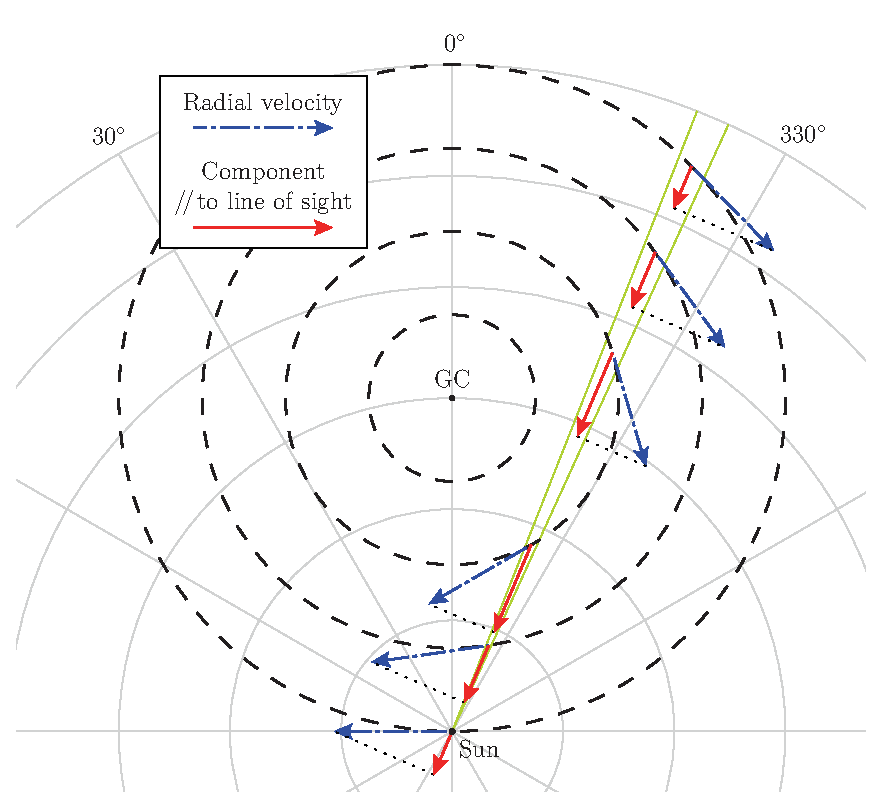
\includegraphics[width = 8cm]{figures/galactic-rotation}
\caption{Galactic rotation showing Doppler shifts}
\label{fig:gal-rot}
\end{figure}

\section{Data analysis}
\paragraph{}
Data analysis is coming first. We talk about many things including how we managed to reduce the nouse in the \texttt{.fits} files we used to make the analysis. Yeas!

\subsection{Noise analsyis}
\paragraph{}
Yes, keem em cumming!!

\section{Results and discussion}
\paragraph{}
This is where we talk aout all the resuts we get from our data analysis, probably a good idea to cover the data analysis first and all of that so that way things make more sense here. Results should relly not even be in here lel.

\subsection{Source candidates}
\paragraph{}
Here are some of the candidates for the gamma ray sources observed.

\subsubsection{HESS J1632-479}
\paragraph{}
Here are the things for this source. Probably include a picture of the source just as a nice ``here is thing''.

\section{Conclusions}
\paragraph{}
Bitch, we concluding now, making the statements that make a conclusion possible to be made with the words and the mouth. Bitch, we're flawless give us good grades.
\end{multicols}

\printbibliography[heading = bibintoc]

\end{document}